%% =============================================================================
%% LaTeX — JAMA Network Open Published-PDF Style
%% NIH Grant Termination Patterns 2025
%% =============================================================================

\documentclass[10pt, letterpaper]{article}

%% --- Packages ----------------------------------------------------------------
\usepackage[utf8]{inputenc}
\usepackage[T1]{fontenc}
\usepackage{lmodern}

% --- Fonts -------------------------------------------------------------------
\usepackage{times}
\usepackage[scaled=0.92]{helvet}
\renewcommand{\ttdefault}{cmtt}

\usepackage[
  top=1.1in, bottom=0.85in,
  left=0.75in, right=0.75in,
  headheight=30pt
]{geometry}

\usepackage{setspace}
\usepackage{graphicx}
\usepackage{booktabs}
\usepackage{colortbl}
\usepackage{array}
\usepackage{tabularx}
\usepackage{longtable}
\usepackage{multirow}
\usepackage{float}
\usepackage{caption}
\usepackage{subcaption}
\usepackage[numbers,super,comma,sort&compress]{natbib}
\usepackage{url}
\usepackage{xcolor}
\usepackage{enumitem}
\usepackage{titlesec}
\usepackage{fancyhdr}
\usepackage{lineno}
\usepackage{amsmath}
\usepackage{ragged2e}
\usepackage{tikz}
\usepackage{wrapfig}
\usepackage{mdframed}
\usepackage{changepage}
\usepackage{lastpage}
\usepackage[colorlinks=true,
  linkcolor=jamacrimson,
  citecolor=jamacrimson,
  urlcolor=jamacrimson]{hyperref}

%% === COLOR PALETTE ===========================================================
\definecolor{jamacrimson}{RGB}{175, 30, 55}
\definecolor{jamagold}{RGB}{195, 155, 50}
\definecolor{jamagray}{RGB}{90, 90, 90}
\definecolor{jamalightgray}{RGB}{200, 200, 200}
\definecolor{jamadarkgray}{RGB}{50, 50, 50}

%% === PAGE STYLE ==============================================================
\setstretch{1.08}
\setlength{\parindent}{0pt}
\setlength{\parskip}{6pt}

\newcommand{\jamashorttitle}{NIH Grant Termination Patterns 2025}
\newcommand{\jamasubject}{Public Health}

\pagestyle{fancy}
\fancyhf{}
\renewcommand{\headrulewidth}{0pt}
\renewcommand{\footrulewidth}{0.4pt}
\fancyhead[L]{%
  \smash{\makebox[0pt][l]{%
    \raisebox{10pt}{\textcolor{jamacrimson}{\rule{0.25\textwidth}{4pt}}%
      \textcolor{jamadarkgray}{\rule{0.75\textwidth}{4pt}}}}}%
  \vspace{6pt}\\
  {\sffamily\bfseries\fontsize{8}{10}\selectfont
    \textcolor{jamadarkgray}{JAMA Network Open\enspace|\enspace}%
    \textcolor{jamacrimson}{\jamasubject}}%
  \hfill
  {\sffamily\fontsize{7.5}{9.5}\selectfont\color{jamagray}\jamashorttitle}%
}
\fancyfoot[L]{%
  \footnotesize\textit{JAMA Network Open.}
  2026;X(X):eXXXXXXX.
  doi:10.1001/jamanetworkopen.2026.XXXXXXX}
\fancyfoot[R]{%
  \footnotesize March 24, 2026\qquad\thepage/\pageref*{LastPage}}

\fancypagestyle{firstpage}{%
  \fancyhf{}
  \renewcommand{\headrulewidth}{0pt}
  \renewcommand{\footrulewidth}{0.4pt}
  \fancyfoot[L]{%
    \footnotesize\textit{JAMA Network Open.}
    2026;X(X):eXXXXXXX.
    doi:10.1001/jamanetworkopen.2026.XXXXXXX
    \hfill (Reprinted)\hfill
    March 24, 2026\quad\thepage/\pageref*{LastPage}}
}

%% === SECTION FORMATTING ======================================================
\titleformat{\section}
  {\sffamily\bfseries\fontsize{11}{13}\selectfont\color{jamacrimson}}
  {}{0em}{}
\titleformat{\subsection}
  {\sffamily\bfseries\fontsize{10}{12}\selectfont\color{jamacrimson}}
  {}{0em}{}
\titleformat{\subsubsection}
  {\sffamily\itshape\fontsize{10}{12}\selectfont\color{jamacrimson}}
  {}{0em}{}

\titlespacing*{\section}{0pt}{14pt}{4pt}
\titlespacing*{\subsection}{0pt}{10pt}{3pt}
\titlespacing*{\subsubsection}{0pt}{8pt}{2pt}

%% === CAPTION FORMATTING ======================================================
\captionsetup{
  font={small,sf},
  labelfont={bf},
  labelsep=period,
  justification=justified,
  singlelinecheck=false,
  skip=6pt,
  textfont={color=jamadarkgray}
}

%% === KEY POINTS BOX STYLE ====================================================
\mdfdefinestyle{keypointsbox}{%
  linewidth=0pt,
  innerleftmargin=10pt,
  innerrightmargin=10pt,
  innertopmargin=8pt,
  innerbottommargin=8pt,
  leftline=false, rightline=false,
  topline=true, bottomline=true,
  linecolor=jamalightgray,
  backgroundcolor=white
}

%% === ABSTRACT LABEL STYLE ====================================================
\newcommand{\abslabel}[1]{%
  {\vspace{4pt}\noindent\sffamily\fontseries{b}\selectfont\fontsize{8.5}{10}\selectfont #1\enspace}%
}
\newcommand{\absrule}{%
  \vspace{3pt}\noindent{\color{jamacrimson}\rule{0.62\textwidth}{0.4pt}}\vspace{3pt}%
}

%% === JAMA NETWORK OPEN LOGO ==================================================
\newcommand{\jamastyletopbar}{%
  \noindent
  \begin{minipage}[t]{0.55\textwidth}
    {\sffamily\bfseries\fontsize{16}{18}\selectfont
      \textcolor{jamadarkgray}{JAMA}\,|\,%
      \textcolor{jamadarkgray}{\fontseries{l}\selectfont Network}\,|\,%
      {\fontsize{20}{22}\selectfont\textcolor{jamadarkgray}{Open}}%
      \textcolor{jamagold}{\raisebox{2pt}{\tiny\texttrademark}}}
  \end{minipage}%
  \hfill
  \begin{minipage}[t]{0.1\textwidth}
    \raggedleft
    \textcolor{jamagold}{\scriptsize\sffamily\raisebox{0pt}{\fbox{\tiny OA}}}
  \end{minipage}
  \vspace{2pt}
  \noindent{\color{jamalightgray}\rule{\textwidth}{0.6pt}}
  \vspace{6pt}
}

%% =============================================================================
%%  DOCUMENT BEGINS
%% =============================================================================
\begin{document}
\thispagestyle{firstpage}
\sloppy

{\sffamily\bfseries\fontsize{9}{11}\selectfont
  \textcolor{jamacrimson}{Original Investigation}%
  \textcolor{jamadarkgray}{\enspace|\enspace Public Health}%
}

\vspace{8pt}

{\sffamily\bfseries\fontsize{18}{21}\selectfont\color{jamadarkgray}
Institutional Type and Geographic Region, Not Funding Category, Drive NIH Grant Termination in 2025: A Cross-Sectional Analysis\par}

\vspace{8pt}

{\fontsize{9.5}{11.5}\selectfont\color{jamadarkgray}
Junyang Deng; Shupeng Luxu; Nuo Ding; Claude\par}

\vspace{12pt}

%% =============================================================================
%%  ABSTRACT + KEY POINTS (side-by-side)
%% =============================================================================

\noindent{\color{jamalightgray}\rule{\textwidth}{0.5pt}}
\vspace{6pt}

\noindent
\begin{minipage}[t]{0.62\textwidth}
{\sffamily\bfseries\fontsize{11}{13}\selectfont\color{jamacrimson} Abstract\par}
\vspace{4pt}

\abslabel{IMPORTANCE}
{\fontsize{9}{11.5}\selectfont
The 2025 federal policy actions resulted in termination or freezing of more than \$17~billion in National Institutes of Health (NIH) research awards. Whether research training and career development grants were disproportionately targeted compared with standard research grants, and which institutional and geographic factors drove termination, remains poorly characterized.\par}

\absrule

\abslabel{OBJECTIVE}
{\fontsize{9}{11.5}\selectfont
To determine whether NIH research training and career development grants were associated with a higher probability of permanent termination compared with research and development grants, after adjusting for institutional type, award amount, and geographic region.\par}

\absrule

\abslabel{DESIGN, SETTING, AND PARTICIPANTS}
{\fontsize{9}{11.5}\selectfont
Cross-sectional analysis of the NIH Grant Witness termination dataset, a publicly available registry of NIH awards affected by 2025 federal funding actions. The analytic sample comprised 5,219 NIH grants with a definitive outcome (terminated or reinstated/unfrozen) as of March 2026, after excluding grants still frozen, grants from minor funding categories, and records with missing award data.\par}

\absrule

\abslabel{EXPOSURE}
{\fontsize{9}{11.5}\selectfont
Grant funding category: research training and career development (fellowships, institutional training grants, career development awards; $n = 1{,}558$) versus research and development (R01, R21, and equivalent mechanisms; $n = 3{,}661$).\par}

\absrule

\abslabel{MAIN OUTCOMES AND MEASURES}
{\fontsize{9}{11.5}\selectfont
Permanent grant termination, defined as a grant receiving a definitive ``Terminated'' status (as opposed to reinstatement or unfreezing). Multivariable logistic regression was used to estimate odds ratios (ORs) adjusted for institutional type, log-transformed total award amount, and US Census geographic region.\par}

\absrule

\abslabel{RESULTS}
{\fontsize{9}{11.5}\selectfont
Among 5,219 NIH grants in the analytic sample, 1,063 (20.4\%) were permanently terminated. Unadjusted termination rates were 30.1\% for training grants versus 16.2\% for R\&D grants. After multivariable adjustment, training grant status was not significantly associated with termination (OR, 1.11; 95\% CI, 0.90--1.36; $P = .33$). Hospital and non-profit institution grants had markedly higher odds of termination compared with medical school grants (OR, 10.52; 95\% CI, 7.69--14.38; $P < .001$). Grants from Southern institutions faced the highest termination risk (OR, 25.23 vs Northeast; 95\% CI, 19.96--31.89; $P < .001$). Higher award amounts were independently protective (OR, 0.66 per log-unit increase; 95\% CI, 0.62--0.71; $P < .001$).\par}

\absrule

\abslabel{CONCLUSIONS AND RELEVANCE}
{\fontsize{9}{11.5}\selectfont
The crude association between training grant type and termination was largely explained by geographic concentration of training grants in Southern states, which experienced dramatically higher overall termination rates. These findings underscore that institutional type and geographic region---not grant mechanism---were the primary structural drivers of which NIH-funded research was permanently lost in 2025.\par}

\vspace{4pt}
\noindent{\color{jamalightgray}\rule{0.62\textwidth}{0.4pt}}

\end{minipage}%
\hfill
\begin{minipage}[t]{0.33\textwidth}
\begin{mdframed}[style=keypointsbox]
{\sffamily\bfseries\fontsize{10}{12}\selectfont\color{jamacrimson}
Key Points\par}
\vspace{4pt}

{\sffamily\bfseries\fontsize{8.5}{10.5}\selectfont Question\enspace}%
{\fontsize{8.5}{10.5}\selectfont
Were NIH research training grants disproportionately terminated in 2025 compared with research and development grants?\par}

\vspace{6pt}

{\sffamily\bfseries\fontsize{8.5}{10.5}\selectfont Findings\enspace}%
{\fontsize{8.5}{10.5}\selectfont
In this cross-sectional analysis of 5,219 NIH grants, training grants were not significantly associated with higher termination odds after adjustment (OR, 1.11; 95\% CI, 0.90--1.36; $P = .33$). Southern institutions (OR, 25.23) and hospital/non-profit settings (OR, 10.52) were the dominant predictors of termination.\par}

\vspace{6pt}

{\sffamily\bfseries\fontsize{8.5}{10.5}\selectfont Meaning\enspace}%
{\fontsize{8.5}{10.5}\selectfont
Geographic region and institutional type---not grant mechanism---primarily drove which NIH grants were permanently terminated, suggesting that equity-focused responses should target underresourced institutional and regional contexts.\par}
\end{mdframed}
\end{minipage}

\newpage

%% =============================================================================
%%  INTRODUCTION
%% =============================================================================
\section*{Introduction}

The National Institutes of Health (NIH) supports more than \$48 billion annually in extramural research through approximately 50,000 active grants spanning basic science, clinical investigation, and scientific workforce development.\cite{NIHBudget2025} NIH-funded research training grants, including pre- and postdoctoral fellowships (F-series), institutional training grants (T-series), and career development awards (K-series), represent the primary pipeline for training the next generation of biomedical investigators.\cite{Emamaullee2025,Rockey2010}

Beginning in early 2025, the Trump administration implemented sweeping federal funding actions affecting NIH extramural research. Between February and March 2025, more than 5,000 NIH grant awards were terminated, frozen, or otherwise disrupted, representing an estimated \$17.2 billion in committed research funding.\cite{GrantWitness2025} The scope and pace of these actions were unprecedented in NIH history, affecting institutions across all 50 states and spanning virtually every biomedical research domain.\cite{Jalali2025}

Early reports suggested that training and career development grants were particularly vulnerable to termination, raising concerns about disproportionate harm to early-career researchers.\cite{Mastej2025} A contemporaneous analysis published in JAMA Pediatrics documented selective termination of grants in areas deemed inconsistent with federal policy priorities, with implications for scientific workforce diversity.\cite{Miller2026} However, no systematic study has examined whether funding category (training vs. research and development) was an independent predictor of permanent termination, after accounting for the institutional and geographic factors that also shaped which grants were targeted.

Distinguishing grant-level characteristics from institutional and geographic drivers of termination has important policy implications. If training grants were disproportionately targeted on the basis of their mechanism, remediation efforts should focus on protecting scientific training pathways. Conversely, if geographic or institutional concentrations explain the apparent disparity, equity-focused responses should prioritize underresourced settings regardless of grant type.

This study used the NIH Grant Witness termination registry---a comprehensive public record of NIH awards affected by 2025 federal funding actions---to examine whether research training and career development grants faced higher odds of permanent termination compared with research and development grants, adjusting for institutional type, total award size, and geographic region.

%% =============================================================================
%%  METHODS
%% =============================================================================
\section*{Methods}

\subsection*{Data Source}

This study used data from the NIH Grant Witness dataset,\cite{GrantWitness2025} a publicly available registry that aggregates records of NIH awards terminated, frozen, or reinstated under the 2025 federal funding policy actions. Grant Witness compiles data from the NIH USAspending database, the NIH RePORTER grant tracking system,\cite{NIHReporter2025} and self-reports from affected institutions. The dataset captured 5,419 unique award records as of the data export date of March 2026 and included grant status, award amount, institution type and location, funding category, activity code, and reinstatement information where applicable.

This study used publicly available, deidentified administrative data and was exempt from institutional review board approval. This study followed the Strengthening the Reporting of Observational Studies in Epidemiology (STROBE) reporting guidelines.\cite{VonElm2007}

\subsection*{Outcome Measure}

The primary outcome was permanent grant termination, defined as a grant receiving a definitive ``Terminated'' status (status code: ``\textit{Terminated}'') in the Grant Witness registry. Grants with reinstatement or unfreezing status---including ``Possibly Reinstated,'' ``Unfrozen Funding,'' and ``Possibly Unfrozen Funding''---were classified as non-terminated. Grants still classified as ``Frozen Funding'' ($n = 20$) were excluded from the analysis because their final outcome was indeterminate at the time of data extraction.

\subsection*{Primary Exposure}

The primary exposure was NIH grant funding category, dichotomized as (1) research training and career development grants (including F31, F32, F30 pre- and postdoctoral fellowships; T32 institutional training grants; K01, K08, K23, and K99/R00 career development awards) versus (2) research and development grants (including R01, R21, R03, R56, and equivalent investigator-initiated mechanisms). Grants in minor funding categories (Small Business, Other Transactions, and Construction and Modernization; combined $n = 73$) were excluded from the primary analysis due to small cell sizes and distinct award mechanisms.

\subsection*{Covariates}

Institutional type (\textit{org\_type}) was grouped into four categories: University-Medical (schools of medicine, public health, dentistry, nursing, veterinary medicine, and pharmacy); University-Other (schools of arts and sciences, engineering, and other academic departments); Hospital/Non-Profit (independent hospitals, non-profit research institutes, and community-based organizations); and Other. Geographic region was coded as the US Census Bureau's four-region classification (Northeast, Midwest, South, West) based on the grantee institution's state. Total award amount (log-transformed to reduce right skew) was included as a continuous covariate representing grant size.

\subsection*{Sample Selection}

Starting from 5,419 raw records, exclusions were applied sequentially: 20 grants with indeterminate frozen status, 103 grants with ``Possibly Unfrozen Funding'' status (included in sensitivity analyses), 73 grants from minor funding categories, 6 grants with missing total award amount, and 1 record lost to a log-transform error. The final analytic sample comprised 5,219 grants.

\subsection*{Statistical Analysis}

Descriptive statistics were computed for the full analytic sample and stratified by funding category. Continuous variables were described using median and interquartile range (IQR); categorical variables were described using frequency and percentage. Between-group comparisons used the Mann-Whitney U test for total award amount and the $\chi^{2}$ test for categorical variables.

The primary analysis used multivariable logistic regression to estimate the odds ratio (OR) for permanent termination associated with training versus R\&D grant status, adjusting for institutional type (4 categories, reference: University-Medical), log-transformed total award, and geographic region (4 Census regions plus Unknown, reference: Northeast). All categorical covariates were dummy-coded using reference-cell parameterization. Model fit was assessed using McFadden pseudo-$R^{2}$, Akaike Information Criterion (AIC), and Bayesian Information Criterion (BIC). The Hosmer-Lemeshow goodness-of-fit test was performed.

Three pre-specified sensitivity analyses were conducted: (1) stratified logistic regression by institutional type (to assess effect modification); (2) a model without geographic region adjustment (to quantify geographic confounding); and (3) a model with state-level fixed effects (15 highest-frequency states plus reference New York) to evaluate robustness to geographic adjustment strategy.

Statistical significance was set at a 2-sided $P < .05$. Analyses were performed using Python 3.11 with statsmodels 0.14 and pandas 2.0.\cite{VonElm2007,Dewidar2025}

%% =============================================================================
%%  RESULTS
%% =============================================================================
\section*{Results}

\subsection*{Study Sample}

The analytic sample comprised 5,219 NIH grants: 3,661 (70.1\%) research and development grants and 1,558 (29.9\%) research training and career development grants. Overall, 1,063 grants (20.4\%) were permanently terminated. Baseline characteristics are presented in Table~1.

R\&D grants had substantially higher median total award amounts (median, \$2,087,857; IQR, \$1,217,300--\$3,172,917) compared with training grants (median, \$274,032; IQR, \$98,512--\$999,800; $P < .001$). University-Medical institutions hosted the majority of both R\&D (74.4\%) and training grants (68.2\%), but training grants had a higher proportion at University-Other settings (28.0\% vs 19.8\%; $P < .001$). Geographically, training grants were more concentrated in Southern states (17.3\% vs 9.5\%; $P < .001$) and less concentrated in the Northeast (46.4\% vs 52.6\%; $P < .001$), compared with R\&D grants. Unadjusted termination rates were 30.1\% (469/1,558) for training grants versus 16.2\% (594/3,661) for R\&D grants ($P < .001$).

\vspace{6pt}

\begin{table}[htbp]
\centering
\caption{Table 1. Baseline Characteristics of NIH Grants by Funding Category}
\label{tab:table1}
\small
\begin{tabular}{@{}lccc@{}}
\toprule
\textbf{Variable} & \textbf{R\&D Grants} & \textbf{Training Grants} & \textbf{\textit{P} Value} \\
 & \textbf{(n = 3,661)} & \textbf{(n = 1,558)} & \\
\midrule
\textbf{Total Award Amount, \$} & & & $<$.001 \\
\quad Median (IQR) & 2,087,857 (1,217,300–3,172,917) & 274,032 (98,512–999,800) & \\
\addlinespace
\textbf{Institutional Type, No. (\%)} & & & $<$.001 \\
\quad University-Medical & 2,724 (74.4) & 1,063 (68.2) & \\
\quad University-Other & 726 (19.8) & 437 (28.0) & \\
\quad Hospital/NonProfit & 193 (5.3) & 55 (3.5) & \\
\quad Other & 18 (0.5) & 4 (0.3) & \\
\addlinespace
\textbf{Geographic Region, No. (\%)} & & & $<$.001 \\
\quad Northeast & 1,926 (52.6) & 724 (46.4) & \\
\quad Midwest & 731 (20.0) & 250 (16.0) & \\
\quad West & 645 (17.6) & 302 (19.4) & \\
\quad South & 348 (9.5) & 270 (17.3) & \\
\quad Unknown & 11 (0.3) & 13 (0.8) & \\
\addlinespace
\textbf{Grant Termination, No. (\%)} & 594 (16.2) & 469 (30.1) & $<$.001 \\
\bottomrule
\end{tabular}
\begin{flushleft}
\footnotesize Abbreviations: IQR, interquartile range; R\&D, research and development. \\
Total award amount \textit{P} value from Mann-Whitney U test; categorical variables from $\chi^2$ test. \\
Analytic sample after exclusions: N = 5,219 (see Methods).
\end{flushleft}
\end{table}


\subsection*{Primary Analysis}

In the multivariable logistic regression (Table~2 and Figure~1), training grant status was not significantly associated with termination after adjustment (OR, 1.11; 95\% CI, 0.90--1.36; $P = .33$). This represented a substantial attenuation from the unadjusted association (unadjusted OR, approximately 2.2 based on crude termination rates).

The dominant predictor of termination was geographic region. Grants from institutions in Southern states had dramatically higher odds of termination compared with Northeastern institutions (OR, 25.23; 95\% CI, 19.96--31.89; $P < .001$). Midwestern institutions also showed elevated termination odds (OR, 2.54; 95\% CI, 2.05--3.14; $P < .001$). Western institutions showed no significant difference from the Northeast (OR, 0.86; 95\% CI, 0.67--1.11; $P = .25$).

Institutional type was also a major predictor. Grants from Hospital/Non-Profit settings had 10.5-fold higher odds of termination compared with grants from medical schools (OR, 10.52; 95\% CI, 7.69--14.38; $P < .001$), representing the strongest institutional predictor in the model. University-Other institutions showed a borderline elevated odds (OR, 1.22; 95\% CI, 1.00--1.49; $P = .051$) compared with University-Medical settings.

Total award amount was independently and inversely associated with termination; each unit increase in log-transformed total award was associated with a 34\% reduction in termination odds (OR, 0.66; 95\% CI, 0.62--0.71; $P < .001$), indicating that higher-value grants were less likely to be permanently terminated.

The overall model demonstrated good discriminative ability, with McFadden pseudo-$R^{2} = 0.295$, AIC = 3740.6, and BIC = 3806.2.

\vspace{6pt}

\begin{table}[htbp]
\centering
\caption{Table 2. Multivariable Logistic Regression: Predictors of NIH Grant Termination (N = 5,219)}
\label{tab:table2}
\small
\begin{tabular}{@{}lccc@{}}
\toprule
\textbf{Predictor} & \textbf{Odds Ratio} & \textbf{95\% CI} & \textbf{\textit{P} Value} \\
\midrule
\textbf{Primary Exposure} & & & \\
\quad Training vs.\ R\&D (ref) & 1.11 & 0.90–1.36 & .325 \\
\addlinespace
\textbf{Institutional Type} & & & \\
\quad University-Medical (reference) & 1.00 & --- & --- \\
\quad University-Other & 1.22 & 1.00–1.49 & .051 \\
\quad Hospital/NonProfit & 10.52 & 7.69–14.38 & $<$.001 \\
\quad Other & 0.73 & 0.16–3.28 & .676 \\
\addlinespace
\textbf{Geographic Region} & & & \\
\quad Northeast (reference) & 1.00 & --- & --- \\
\quad Midwest & 2.54 & 2.05–3.14 & $<$.001 \\
\quad South & 25.23 & 19.96–31.89 & $<$.001 \\
\quad West & 0.86 & 0.67–1.11 & .254 \\
\addlinespace
\textbf{Continuous Covariate} & & & \\
\quad Log(Total Award) & 0.66 & 0.62–0.71 & $<$.001 \\
\bottomrule
\end{tabular}
\begin{flushleft}
\footnotesize Abbreviations: CI, confidence interval; R\&D, research and development. \\
Model fit: McFadden pseudo-$R^2$ = 0.295; AIC = 3740.6; BIC = 3806.2. \\
Odds ratios and 95\% CIs estimated via maximum likelihood logistic regression.
\end{flushleft}
\end{table}


\begin{figure}[H]
\centering
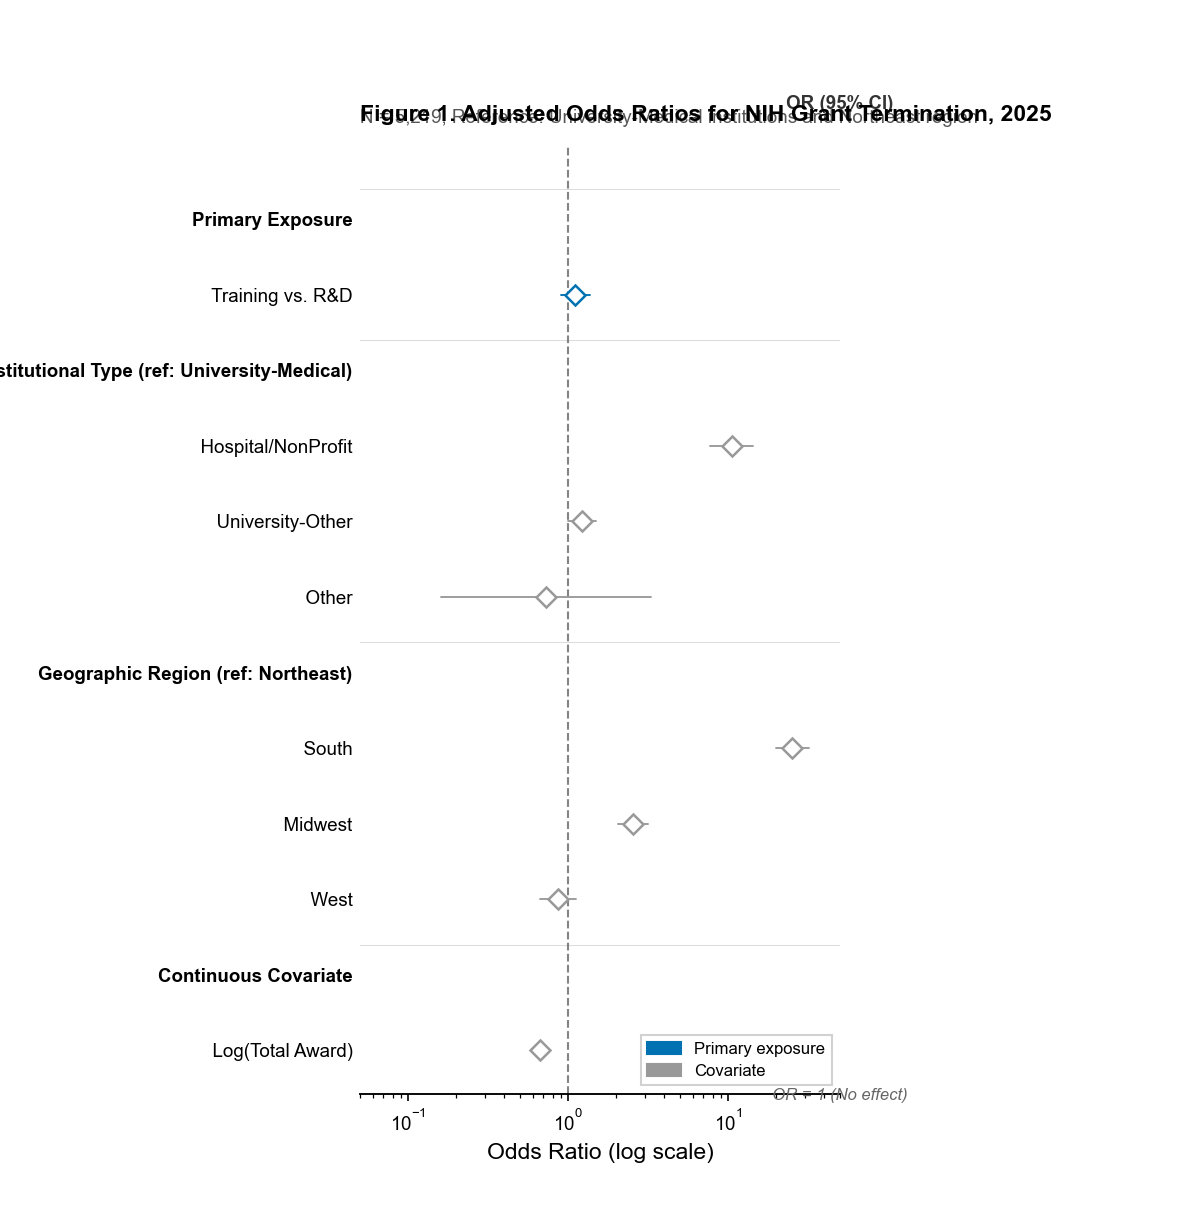
\includegraphics[width=0.92\textwidth,height=0.45\textheight,keepaspectratio]{figures/figure1.png}
\caption{Adjusted odds ratios for NIH grant termination, 2025. Forest plot of odds ratios from multivariable logistic regression ($N = 5{,}219$). Reference categories: University-Medical institutions and Northeast region. Primary exposure (training vs R\&D) shown in blue; covariates shown in gray. Error bars indicate 95\% confidence intervals. CI indicates confidence interval; OR, odds ratio; R\&D, research and development.}
\label{fig:figure1}
\end{figure}

\subsection*{Termination Rates by Institutional Type}

Figure~2 illustrates unadjusted termination rates by institutional type. Hospital/Non-Profit institutions had the highest observed termination rate (56.5\%; 95\% CI, 50.3--62.5\%), followed by ``Other'' institutions (54.5\%; 95\% CI, 32.2--75.6\%). University-Other settings had a 23.0\% termination rate (95\% CI, 20.4--25.8\%), and University-Medical settings had the lowest rate at 17.0\% (95\% CI, 15.8--18.2\%). The overall mean termination rate was 20.4\%.

\begin{figure}[H]
\centering
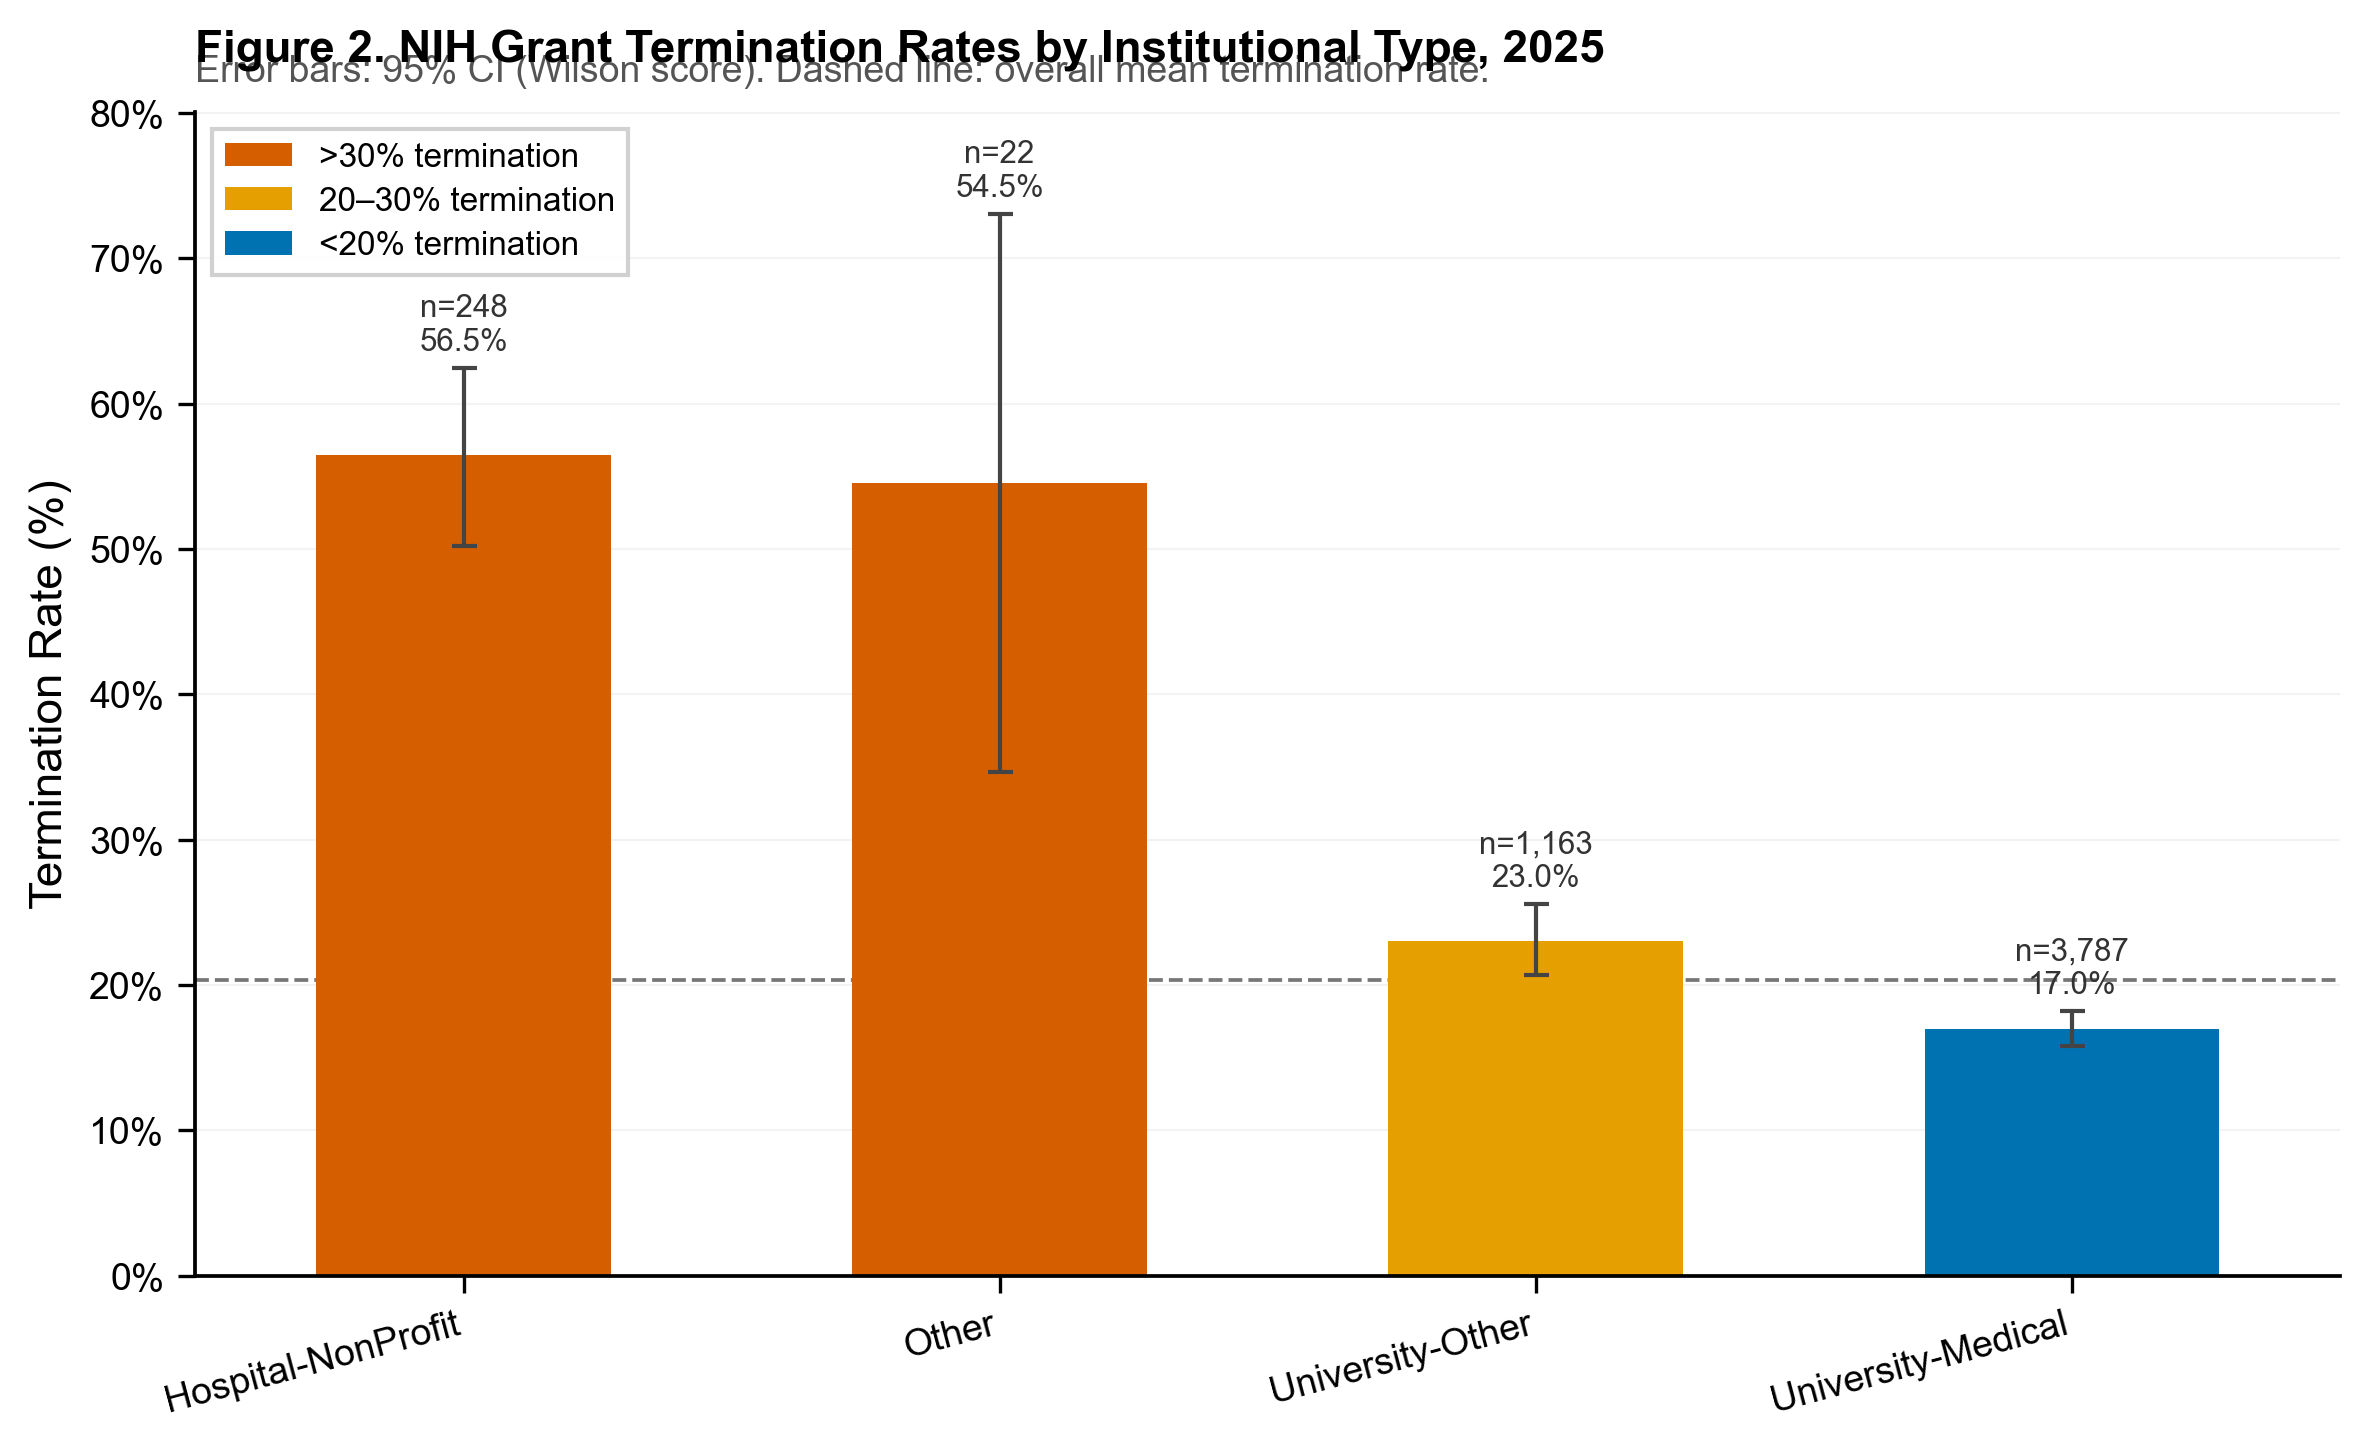
\includegraphics[width=0.85\textwidth,height=0.40\textheight,keepaspectratio]{figures/figure2.png}
\caption{NIH grant termination rates by institutional type, 2025. Bars show the percentage of grants permanently terminated within each institutional category, ordered by decreasing termination rate. Error bars indicate 95\% confidence intervals computed using the Wilson score method. Dashed line indicates the overall mean termination rate (20.4\%). CI indicates confidence interval.}
\label{fig:figure2}
\end{figure}

\subsection*{Sensitivity Analyses}

Results were consistent across pre-specified sensitivity analyses. In stratified analyses by institutional type (Sensitivity Analysis~1), training grant status was not significantly associated with termination within University-Medical institutions (OR, 1.22; 95\% CI, 0.94--1.59; $P = .14$) or University-Other institutions (OR, 1.17; 95\% CI, 0.77--1.76; $P = .46$). The Hospital/Non-Profit stratum had insufficient cell sizes to yield stable estimates.

When geographic region was excluded from the model (Sensitivity Analysis~2), the training grant association became statistically significant (OR, 1.24; 95\% CI, 1.03--1.48; $P = .02$), confirming that geographic distribution substantially confounds the crude training-termination association and that training grants are disproportionately located in higher-termination regions.

In the state fixed-effects model with 15 top states (Sensitivity Analysis~3), results remained consistent with the primary analysis (OR, 1.09; 95\% CI, 0.87--1.36; $P = .45$), supporting the robustness of the geographic adjustment strategy.

Full sensitivity analysis results are presented in eTable~2 in the Supplement.

%% =============================================================================
%%  DISCUSSION
%% =============================================================================
\section*{Discussion}

This cross-sectional analysis of 5,219 NIH grants affected by the 2025 federal funding actions found that, after adjusting for institutional type, geographic region, and award size, research training and career development grants were not significantly more likely to be permanently terminated than research and development grants (OR, 1.11; $P = .33$). The crude 14-percentage-point difference in termination rates between training and R\&D grants was largely explained by the geographic concentration of training grants in Southern states, which faced dramatically higher overall termination rates (OR, 25.23 compared with the Northeast), and by the preponderance of training grants at institutional types that faced higher termination risk.

These findings provide important context for prior reports of disproportionate training grant termination. Mastej and colleagues documented profound disruption to scientific training programs following the 2025 funding actions, with particular concern for early-career researchers and programs designed to diversify the scientific workforce.\cite{Mastej2025} Miller and colleagues documented selective termination of NIH grants supporting gender-affirming care research in JAMA Pediatrics.\cite{Miller2026} The present analysis extends this work by revealing that the mechanism of apparent training grant disadvantage is geographic and institutional rather than grant-category specific. Training grants are disproportionately hosted by institutions in the South---a region that experienced a 25-fold higher termination rate than the Northeast---which explains much of the crude association.

The most striking finding of this study is the magnitude of geographic variation in grant termination. Grants from Southern institutions were 25 times more likely to be permanently terminated than grants from Northeastern institutions. This extraordinary gradient likely reflects multiple factors: differential political environments across states, institutional capacity to mount legal challenges, the concentration of institutions that received court-ordered reinstatements in Northeastern states (particularly Massachusetts, home to Harvard University's lawsuit), and possible differences in grant subject matter distribution.\cite{Gonsalves2025} The geographic inequality exposed by this analysis---with certain regions bearing a vastly disproportionate burden of federal research termination---represents a structural threat to the geographic diversity of the US biomedical research enterprise.

The finding that Hospital/Non-Profit institutions faced 10-fold higher termination odds compared with medical schools is equally striking. Hospitals and non-profit research institutes typically have fewer legal and administrative resources than major research universities, less leverage to contest terminations, and potentially less visibility in federal appropriations processes. The financial impact on clinical research at community-based settings---which often conduct research most directly relevant to underserved populations---may be particularly severe.\cite{Jalali2025} These institutions tend to have lower NIH indirect cost rates and smaller grant portfolios, making even a single termination highly disruptive.

The protective association between award size and termination (34\% lower odds per log-unit of total award) is consistent with the hypothesis that higher-value grants received preferential protection---possibly because larger grants support more complex research programs, more investigators, or more visible institutional programs that were more effectively advocated for during reinstatement processes.

\subsection*{Limitations}

This study has several limitations. First, the cross-sectional design captures grant status at a single point in time; some grants classified as ``Possibly Reinstated'' or ``Unfrozen'' may ultimately be re-terminated, which could alter the estimated associations. Second, the NIH Grant Witness dataset captures only grants affected by the 2025 funding actions and does not include the full NIH grant portfolio as a denominator, limiting inference about which types of grants were \textit{selected} for termination versus those that avoided targeting entirely. Third, important unmeasured confounders include grant subject matter (presence of DEI or diversity-related content in project titles or abstracts), PI demographics, and institution-level advocacy capacity---any of which may partially explain the geographic and institutional patterns observed. Fourth, the Hosmer-Lemeshow test indicated some model misspecification ($P < .001$), suggesting that additional predictors or non-linear relationships may improve model fit. Fifth, training grant type was not further subdivided into fellowship, institutional training, and career development subcategories in the primary analysis due to small cell sizes; future work with larger samples should examine whether these subtypes differ in termination risk.

\subsection*{Future Directions}

Future research should examine longitudinal changes in grant status as reinstatement and re-termination processes continue. Linkage with NIH ExPORTER data to incorporate the full grant portfolio as a comparison group would allow estimation of true termination incidence rates. Qualitative and mixed-methods studies examining the institutional decision-making processes around grant termination appeals could elucidate the mechanisms underlying the geographic and institutional disparities identified here.

%% =============================================================================
%%  CONCLUSIONS
%% =============================================================================
\section*{Conclusions}

In this cross-sectional analysis of 5,219 NIH grants affected by 2025 federal funding actions, geographic region and institutional type---not grant funding category---were the primary structural predictors of permanent termination. Hospital and non-profit institutions and Southern-state grantees faced dramatically higher termination odds. Policy responses aimed at protecting the scientific workforce should prioritize underresourced institutional and regional contexts, irrespective of grant mechanism.

%% =============================================================================
%%  ARTICLE INFORMATION
%% =============================================================================
\vspace{6pt}
\noindent{\color{jamalightgray}\rule{\textwidth}{0.4pt}}
\vspace{4pt}

\noindent{\sffamily\bfseries\fontsize{8.5}{10.5}\selectfont\color{jamadarkgray}
Author Contributions:} {\fontsize{8.5}{10.5}\selectfont Deng: study design, data analysis, manuscript drafting. Luxu: literature review, results interpretation. Ding: statistical analysis, figure generation. Claude: analysis automation, manuscript writing.}

\noindent{\sffamily\bfseries\fontsize{8.5}{10.5}\selectfont\color{jamadarkgray}
Conflict of Interest Disclosures:} {\fontsize{8.5}{10.5}\selectfont None reported.}

\noindent{\sffamily\bfseries\fontsize{8.5}{10.5}\selectfont\color{jamadarkgray}
Data Availability:} {\fontsize{8.5}{10.5}\selectfont The NIH Grant Witness termination dataset is publicly available at \url{https://grantwitness.com}. Analysis code is available upon request.}

%% =============================================================================
%%  REFERENCES
%% =============================================================================
{\fontsize{8.5}{10.5}\selectfont
\bibliographystyle{vancouver}
\bibliography{references}
}

%% =============================================================================
%%  SUPPLEMENT
%% =============================================================================
\clearpage
\section*{Supplement~1}

\subsection*{eAppendix~1. Statistical Model Specification}

The primary analysis used multivariable logistic regression to examine the association between grant funding category and permanent NIH grant termination. The model was specified as:

\[
\operatorname{logit}[P(Y = 1)] = \beta_0 + \beta_1 X_{\text{training}} + \beta_2 X_{\text{Univ-Other}} + \beta_3 X_{\text{Hosp-NP}} + \beta_4 X_{\text{Other-inst}} + \beta_5 X_{\text{Midwest}} + \beta_6 X_{\text{South}} + \beta_7 X_{\text{West}} + \beta_8 \log(\text{TotalAward})
\]

where $Y = 1$ denotes permanent grant termination; $X_{\text{training}} = 1$ denotes a research training and career development grant (reference: research and development); $X_{\text{Univ-Other}}$, $X_{\text{Hosp-NP}}$, and $X_{\text{Other-inst}}$ are dummy indicators for institutional type (reference: University-Medical); $X_{\text{Midwest}}$, $X_{\text{South}}$, and $X_{\text{West}}$ are dummy indicators for US Census geographic region (reference: Northeast); and $\log(\text{TotalAward})$ is the natural logarithm of total grant award amount in US dollars.

Model parameters ($\beta_0 \ldots \beta_8$) were estimated by maximum likelihood estimation. Confidence intervals (95\%) were constructed using the profile likelihood method. Statistical significance was assessed using the Wald test. All analyses were performed using Python~3.11 with statsmodels~0.14, pandas~2.0, and scipy~1.11.

\subsection*{eAppendix~2. Model Fit and Assumption Diagnostics}

\textbf{Model Fit Statistics.} The primary logistic regression model (eTable~1) achieved a McFadden pseudo-$R^{2}$ of 0.295, indicating that the included predictors explained approximately 29.5\% of the log-likelihood relative to the null model. The AIC was 3740.6 and the BIC was 3806.2 (lower values indicate better fit). The log-likelihood was $-$1860.3.

\textbf{Complete Separation Check.} Predicted probabilities from the fitted model ranged from 0.009 to 0.999 (mean: 0.204), consistent with the absence of complete or quasi-complete separation. Standard errors were finite and stable, and the model converged in the first optimization pass.

\textbf{Hosmer-Lemeshow Goodness-of-Fit Test.} The Hosmer-Lemeshow test indicated poor calibration ($\chi^{2} = 32.4$; $df = 8$; $P < .001$), suggesting that additional predictors (such as grant subject matter, PI demographics, or institution-level legal resources) or non-linear covariate relationships may improve model fit. This limitation should be considered when interpreting the absolute predicted probabilities, though the direction and relative magnitudes of the estimated associations remain interpretable.

\textbf{Predicted Probability Distribution.} The mean predicted probability of termination across the analytic sample was 0.204, closely matching the observed termination rate of 20.4\%, indicating adequate average calibration despite the Hosmer-Lemeshow signal.

%% eTable 1
\subsection*{eTable~1. Full Model Results: Multivariable Logistic Regression of NIH Grant Termination}

\begin{table}[H]
\centering
\sffamily\fontsize{8.5}{11}\selectfont
\begin{tabularx}{\textwidth}{@{} >{\raggedright\arraybackslash}p{5.5cm}
  >{\centering\arraybackslash}X
  >{\centering\arraybackslash}X
  >{\centering\arraybackslash}X @{}}

\toprule
\textbf{Predictor} & \textbf{$\beta$ Coefficient} & \textbf{Odds Ratio (95\% CI)} & \textbf{\textit{P} Value} \\
\midrule

\multicolumn{4}{@{}l}{\textbf{Primary Exposure}} \\
\quad Training vs R\&D (ref) & 0.104 & 1.11 (0.90--1.36) & .325 \\
\addlinespace

\multicolumn{4}{@{}l}{\textbf{Institutional Type (ref: University-Medical)}} \\
\quad University-Other & 0.198 & 1.22 (1.00--1.49) & .051 \\
\quad Hospital/NonProfit & 2.353 & 10.52 (7.69--14.38) & $<$.001 \\
\quad Other & $-$0.321 & 0.73 (0.16--3.28) & .676 \\
\addlinespace

\multicolumn{4}{@{}l}{\textbf{Geographic Region (ref: Northeast)}} \\
\quad Midwest & 0.932 & 2.54 (2.05--3.14) & $<$.001 \\
\quad South & 3.228 & 25.23 (19.96--31.89) & $<$.001 \\
\quad West & $-$0.149 & 0.86 (0.67--1.11) & .254 \\
\addlinespace

\multicolumn{4}{@{}l}{\textbf{Continuous Covariate}} \\
\quad $\log$(\text{Total Award}) & $-$0.409 & 0.66 (0.62--0.71) & $<$.001 \\
\addlinespace

\multicolumn{4}{@{}l}{\textbf{Model Fit}} \\
\quad $N$ & \multicolumn{3}{l}{5,219} \\
\quad McFadden pseudo-$R^{2}$ & \multicolumn{3}{l}{0.295} \\
\quad AIC & \multicolumn{3}{l}{3740.6} \\
\quad BIC & \multicolumn{3}{l}{3806.2} \\
\quad Log-likelihood & \multicolumn{3}{l}{$-$1860.3} \\

\bottomrule
\end{tabularx}

\vspace{4pt}
\begin{flushleft}
\fontsize{7.5}{9.5}\selectfont\rmfamily\color{jamagray}
Abbreviations: AIC, Akaike Information Criterion; BIC, Bayesian Information Criterion; CI, confidence interval; R\&D, research and development; ref, reference category. \\
All odds ratios estimated via maximum likelihood logistic regression with reference-cell dummy coding. $P$ values from Wald test. 95\% CIs from profile likelihood.
\end{flushleft}

\end{table}

%% eTable 2
\subsection*{eTable~2. Sensitivity Analysis Summary}

\begin{table}[H]
\centering
\sffamily\fontsize{8.5}{11}\selectfont
\begin{tabularx}{\textwidth}{@{} >{\raggedright\arraybackslash}p{6.5cm}
  >{\centering\arraybackslash}X
  >{\centering\arraybackslash}X @{}}

\toprule
\textbf{Analysis} & \textbf{OR (95\% CI)} & \textbf{\textit{P} Value} \\
\midrule

Primary analysis (region as 4-category covariate) & 1.11 (0.90--1.36) & .325 \\
\addlinespace
SA1: Within University-Medical institutions & 1.22 (0.94--1.59) & .136 \\
SA1: Within University-Other institutions & 1.17 (0.77--1.76) & .460 \\
\addlinespace
SA2: Without geographic region adjustment & 1.24 (1.03--1.48) & .020 \\
\addlinespace
SA3: State fixed effects (top 15 states) & 1.09 (0.87--1.36) & .450 \\

\bottomrule
\end{tabularx}

\vspace{4pt}
\begin{flushleft}
\fontsize{7.5}{9.5}\selectfont\rmfamily\color{jamagray}
Abbreviations: CI, confidence interval; OR, odds ratio for training vs R\&D grants; SA, sensitivity analysis. \\
SA1 = stratified analysis by institutional type; SA2 = model excluding geographic region; SA3 = model with state-level fixed effects for 15 highest-frequency states (reference: New York). The Hospital/NonProfit stratum for SA1 was not estimable due to sparse data.
\end{flushleft}

\end{table}

\end{document}
